\begin{savequote}[75mm]
This is some random quote to start off the chapter.
\qauthor{Firstname lastname}
\end{savequote}

\chapter{The ATLAS detector and the Large Hadron Collider}

This chapter presents an overview of the experimental systems used to conduct the measurements presented in this thesis. First, a brief overview of the accelerator, the Large Hadron Collider, will be given. In this section, the accelerator conditions relevant to data-taking are presented as well. Next, an overview of the ATLAS experiment is given. The basics of each sub-detector's role are summarized, as well as the details of the datasets accumulated. Then, a brief interlude on the ATLAS Muon New Small Wheel upgrade is presented. While this new detector does not have a direct impact on any of the datasets taken so far, it will have an impact on future analyses and the work done on it is briefly summarized here. Finally, an overview of object reconstruction in ATLAS is given. While the details of all of the algorithms will not be presented in detail, aspects of the reconstruction performance such as object resolutions are shown as these are relevant to the two studies presented later in this thesis. 

\section{The Large Hadron Collider}

The Large Hadron Collider (LHC) is a proton-proton collider at the CERN laboratory in Geneva, Switzerland\cite{LHCPaper}. It is designed for a maximum collision center of mass energy of $\sqrt{s} = 14 \TeV$ and has a circumference of $26.7$ kilometers. Four main experiments are located at the interaction points (IP) of the accelerator: ATLAS (A Toroidal LHC ApparatuS), CMS (the Compact Muon Solenoid), ALICE (A Large Ion Collider Experiment), and LHC$b$~\cite{ATLASPaper, CMSPaper, LHCbPaper, ALICEPaper}. The studies performed in this thesis were all completed with the ATLAS detector.

Figure~\ref{fig:LHC} shows a schematic of the LHC ring and the various experiments.  

\begin{figure}[h!]
  %\vspace{20pt}
  \centering
  \captionsetup{justification=centering}

  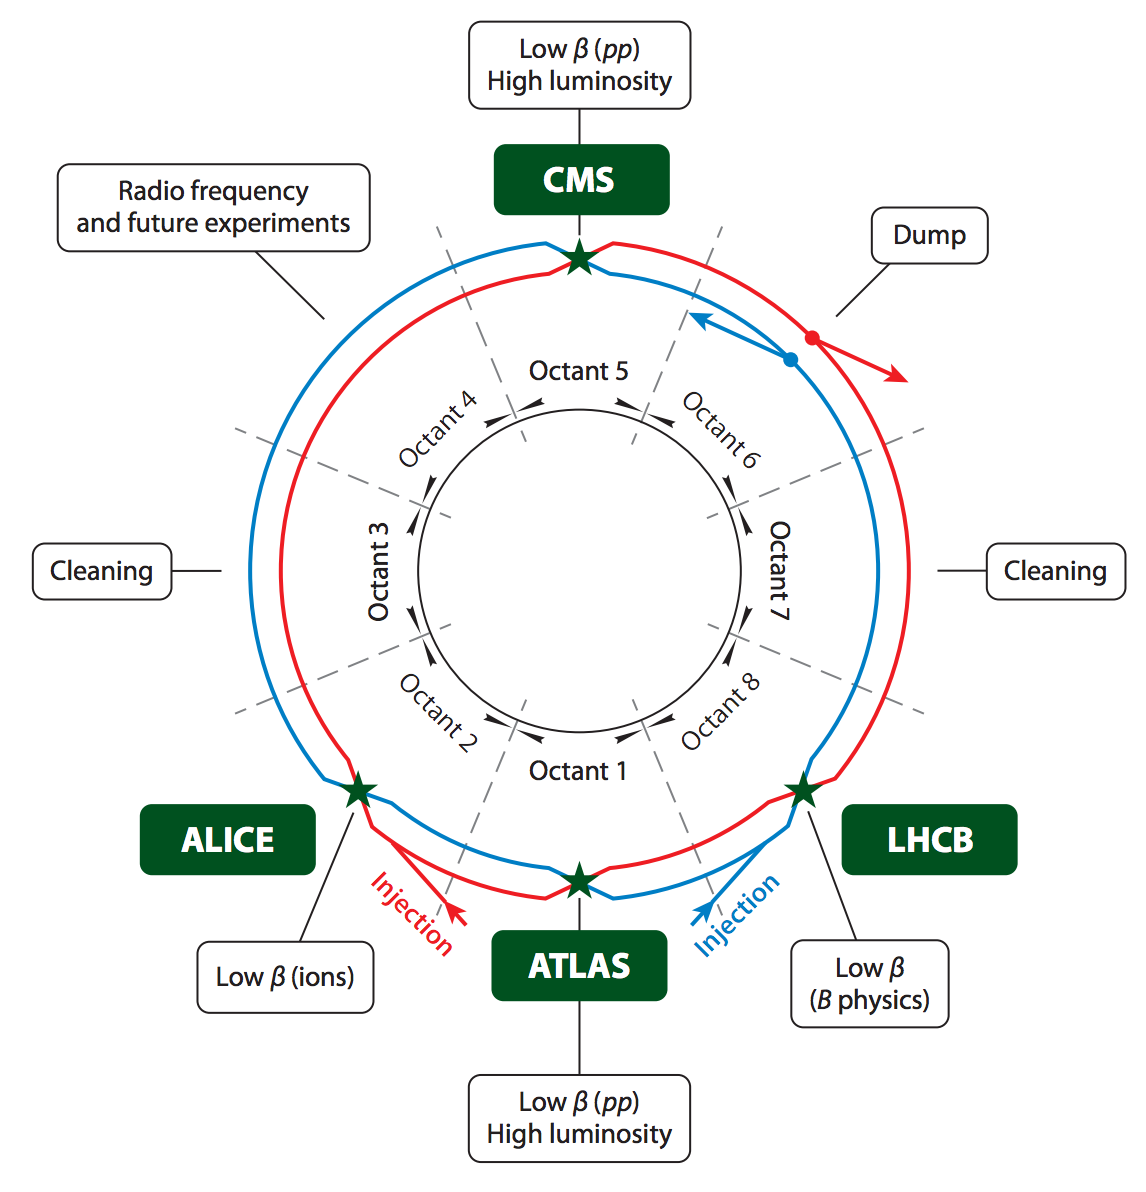
\includegraphics[width=0.7\textwidth]{figures/LHC}
   \caption{A schematic view of the LHC ring ~\cite{LHCReview}}
  \label{fig:LHC}
\end{figure}

One of the most interesting features of the LHC is in its magnet design. Because the tunnel does not have room for separate superconducting magnets for each of the beam pipes, the LHC employs a twin-bore magnet design. Each magnet must hold an $8.3$ Tesla magnetic field in order to bend the proton beams at $\sqrt{s} = 14 \TeV$. The superconducting magnets are cooled to a temperature of $1.9$ Kelvin with superfluid helium.  

\subsection{Instantaneous luminosity}

The rate of physics events expected from the accelerator is dependent on the instantaneous luminosity of the machine and the cross section of the physics process, $R_{\rm events} = L\sigma$. Here, $R_{\rm events}$ is the number of events per second, $L$ is the instantaneous luminosity of the machine, and $\sigma$ is the cross section for the physics process being measured. The instantaneous luminosity of the LHC is determined by numerous factors related to machine conditions. Equation~\ref{eqn:lumi} gives the equation for instantaneous luminosity of Gaussian beam profile~\cite{LHCReview}.

\begin{equation}
\label{eqn:lumi}
L = \frac{N_b^2 n_b f_{\rm rev} \gamma_r}{4\pi \epsilon_n \beta^*} F
\end{equation}

The LHC collides protons in bunches, and in the above equation $N_b$ is the number of protons per bunch while $n_b$ is the number of bunches per beam. Nominally, the LHC can hold up to $2808$ proton bunches. $f_{\rm rev}$ is the revolution frequency. $\epsilon_n$ is the normalized transverse beam emittance, a measurement of the average spread of the particles position-momentum space which has the dimension of length. $\beta^*$ is the value of the $beta$ function for the beam at the interaction point. It relates the emmitance to the Gaussian width of the beam with $\sigma_{\rm beam} = \sqrt{\epsilon \cdot \beta}$. $F$ is a reduction factor that corrects for the fact that the beams are colliding at an angle at the IP. 

Another way of writing the instantaneous luminosity is shown in equation~\ref{eqn:lumi2}. In this case, the instantaneous luminosity is written as the ratio of the rate of inelastic collisions with the inelastic cross section\cite{lumi-paper}. 

\begin{equation}
\label{eqn:lumi2}
L = \frac{R_{\rm inel}}{\sigma_{\rm inel}} = \frac{\mu n_b f_{\rm rev}}{\sigma_{\rm inel}}
\end{equation}

In this case, $\mu$ is the average number of interactions per bunch crossing in the accelerator. $\mu$ is a useful parameter for characterizing the amount of activity recorded in an experiment. As the instantaneous luminosity and thus $\mu$ increase, there are more interactions per bunch crossing and more activity in the detector. This is often characterized with $\langle \mu \rangle$, the measured per bunch crossing $\mu$ value averaged over all bunch crossings. The interactions inside each bunch crossing that are not the main physics process of interest are often referred to as ``pileup" interactions, and $\langle \mu \rangle$ is a measurement of the level of pileup in the detector. 

\subsection{Evolution of machine conditions}

This thesis uses datasets taken at three different center of mass energies: $\sqrt{s} = 7 \TeV$ data taken in the year $2011$, $\sqrt{s} = 8 \TeV$ data taken in the year $2012$, and $\sqrt{s} = 13 \TeV$ dataa taken in the year $2015$. In addition to increasing center of mass energy, the instananeous luminosity and parameters that determine it were evolving. Table~\ref{tab:LHC_cond} summarizes that machine conditions in each of these datasets. 

\begin{table}[h!]
\centering
\captionsetup{justification=centering}

%\begin{tabular*}{0.480\textwidth}{p{0.075\textwidth} p{0.180\textwidth} l}
\hspace{-10pt}
\begin{tabular}{|c|c|c|c|c|}
\hline
& $2011$ & $2012$ & $2015$ & Design\\ \hline
$\sqrt{s}$ [$\TeV$] & $7$ & $8$ & $13$ & $14$ \\ \hline
Number of bunches & $1380$ & $1380$ & $1825$ & $2808$ \\ \hline
Max. protons per bunch & $1.45\times10^{11}$ & $1.7\times10^{11}$ & & $1.15 \times 10^{11}$ \\ \hline
Bunch spacing [$\textrm{ns}$] & $50$ & $50$ & $25$ & $25$ \\ \hline
\specialcell{Max. instantaneous \\ luminosity [$\textrm{cm}^{-2} \textrm{s}^-1$]} & $3.7\times 10^{33}$ & $7.7\times10^{33}$ & $5\times10^{33}$ & $10^{34}$\\ \hline
$\beta^*$ [$\textrm{m}$] & $1.0$ & $0.6$ & $0.8$ & $0.55$ \\ \hline 
$\langle \mu \rangle$ & $11.6$ & $20.7$ & $13.7$ & - \\ \hline
\end{tabular}

\caption{
Evolution of LHC machine conditions~\cite{LHC_2011_2012,LHC_2015}
}
\label{tab:LHC_cond}
\end{table}


\section{The ATLAS Detector}

The ATLAS detector is a multi-purpose particle detector experiment at the LHC's Point $1$~\cite{ATLASPaper}. It has nearly $4\pi$ coverage in solid angle around the interaction point. It consists of an inner detector for measuring charged particles, electromagnetic and hadronic calorimeters, and a muon spectrometer. Figure~\ref{fig:ATLAS_overview} gives an overview of the detector.

\begin{figure}[h!]
  %\vspace{20pt}
  \centering
  \captionsetup{justification=centering}

  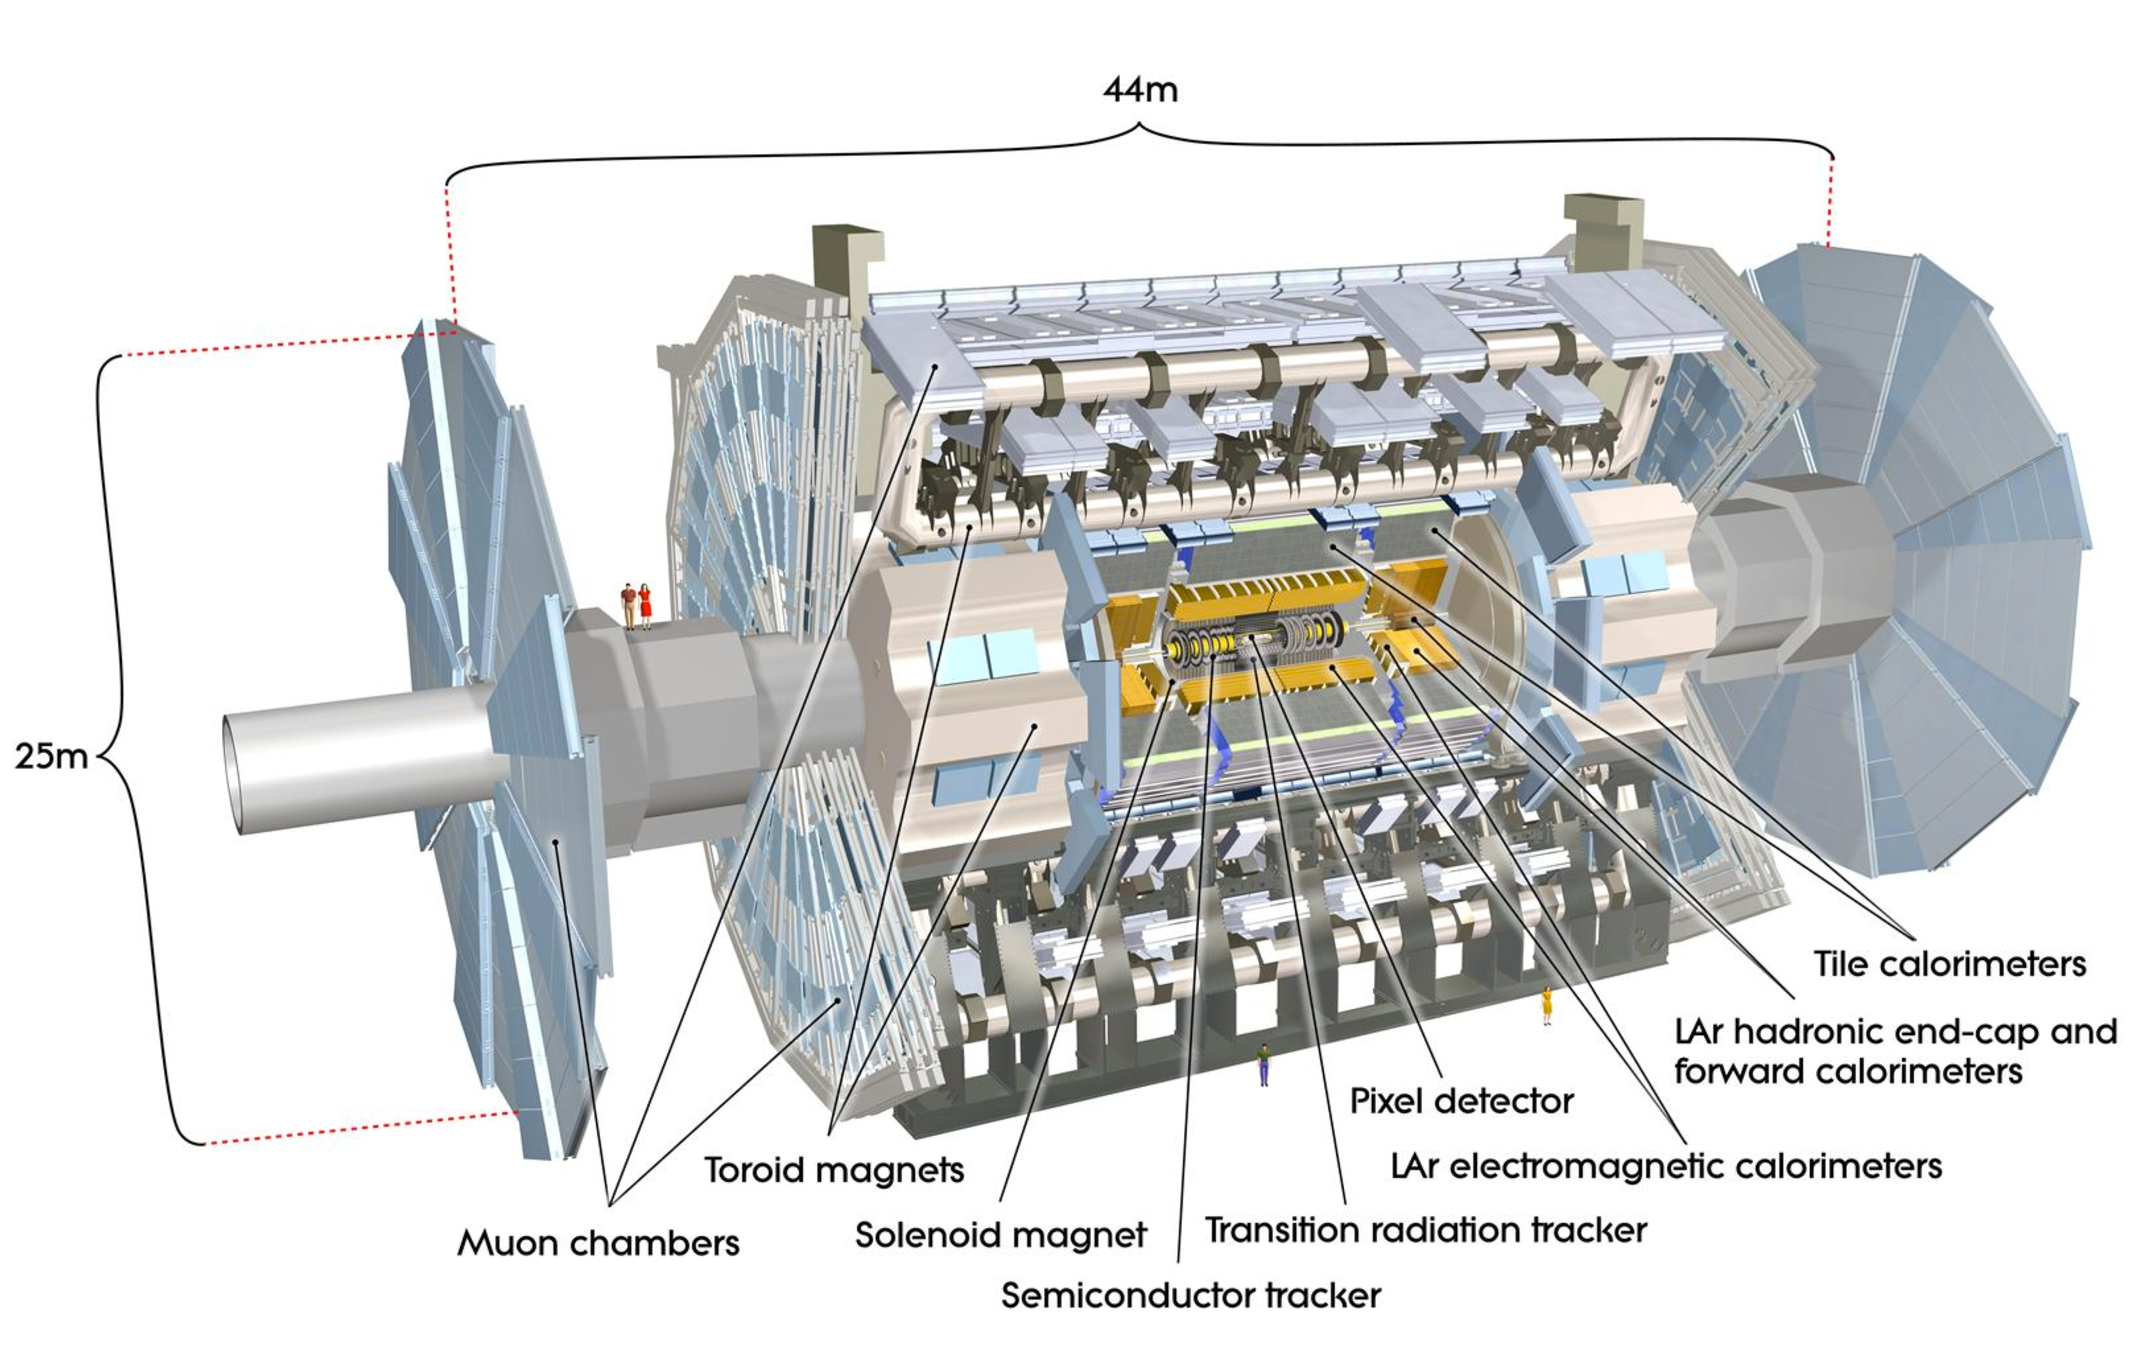
\includegraphics[width=\textwidth]{figures/ATLAS}
   \caption{A full diagram of the ATLAS detector~\cite{ATLASPaper}}
  \label{fig:ATLAS_overview}
\end{figure}

\subsection{Coordinate system}

Before defining the properties of the individual detectors, it is important to establish the coordinate system used. Figure~\ref{fig:coord} shows a schematic of the coordinate system. The azimuthal plane (perpendicular to the beam line) is defined as the $x$-$y$ plane. The angle in this plane is referred to as $\phi$. The angle relative to the beam axis is referred to as $\theta$. Rather than using $\theta$ directly as a coordinate, the experiment often uses the pseudorapidity $\eta$. $\eta$ is defined in equation~\ref{eqn:eta}. 

\begin{equation}
\label{eqn:eta}
\eta = \ln{\left(\tan\left(\frac{\theta}{2}\right)\right)}
\end{equation}

Pseudorapidity is the massless approximation of rapidity, the angle used to paramaterize boosts in special relativity. This is important for two reasons. First, it means that differences in $\eta$ are Lorentz invariant. Second, particle production is roughly constant in pseudorapidity. Particles with $\eta$ close to zero are referred to as ``central", while those at high $|\eta|$ are called ``forward". In general, two main detector topologies can be seen in figure~\ref{fig:ATLAS_overview}. There are ``barrel" elements, which surround the beam line cylindrically and are in the central region of the detector. In the forward region, there are ``endcap" regions which are arranged as disks perpendicular to the beam line. 

\begin{figure}[h!]
  %\vspace{20pt}
  \centering
  \captionsetup{justification=centering}

  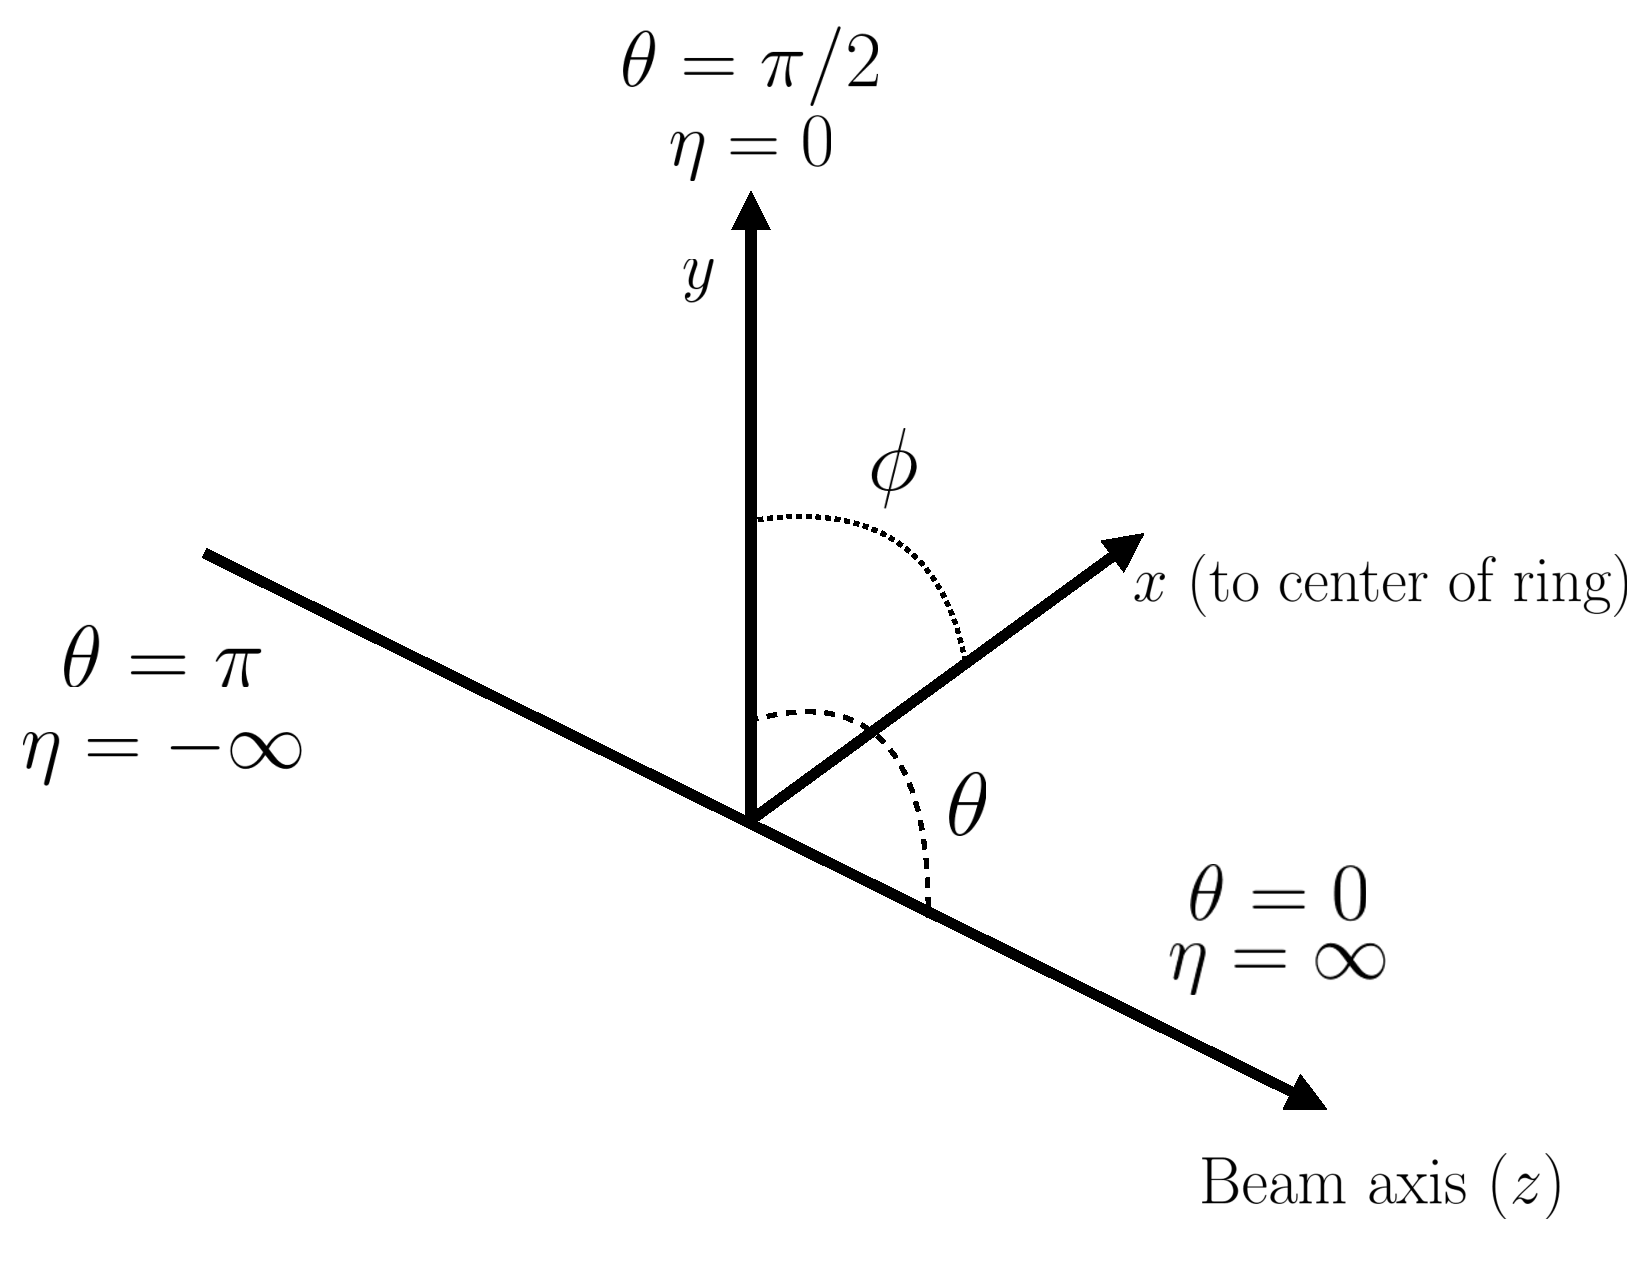
\includegraphics[width=0.8\textwidth]{figures/ATLAS_coord}
   \caption{The ATLAS coordinate system}
  \label{fig:coord}
\end{figure}

\subsection{Inner detector}

The ATLAS Inner Detector (ID) system is built for precision tracking of charged particles. It covers the range $|\eta| < 2.5$. In this range, approximately $1000$ particles are generated every bunch crossing in the detector. This requires having fine granularity to achieve the resolutions required for good momentum measurement and vertex reconstruction. 

The ID consists of three sub-components: the pixel detector, semiconductor tracker (SCT), and transition radiation tracker (TRT). It is surrounded by a solenoid providing a $2$ $\rm T$ axial magnetic field which bends particles in the transverse plane to allow for momentum measurement. Figure~\ref{fig:ID}shows the layout of each of these components. 

\begin{figure}[h!]
  %\vspace{20pt}
  \centering
  \captionsetup{justification=centering}

  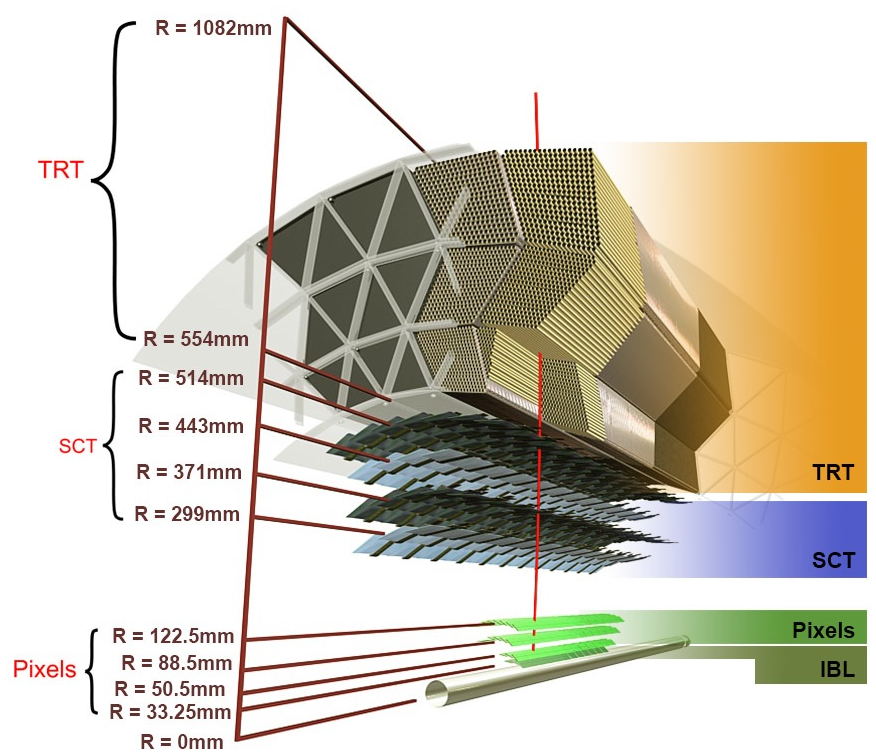
\includegraphics[width=0.7\textwidth]{figures/ATLAS_ID}
   \caption{Layout of the ATLAS Inner Detector system~\cite{Run2Tracking}}
  \label{fig:ID}
\end{figure}

\subsubsection{Pixel detector}

The pixel detector is the first detector particles traverse after being generated in proton collisions and is the most granular detector. Its operation is crucial for precision tracking and vertex reconstruction as well as higher level object reconstruction like tagging of jets from $b$-quarks. The basic sensing element in this subdetector is a silicon pixel detector. The operating principle for the silicon pixels is that of a $p$-$n$ junction. When a charged particle passes through, it creates electron-hole pairs that are then separated by the electric field. The sensors are $250\,\mu\rm m$ thick and use oxygenated $n$-type wafers with readout pixels on the $n^+$ side of the detector~\cite{ATLASPaper}. Overall, the pixel detector has $1744$ sensors and $~80.4$ million readout channels.

In the barrel region, the pixel detector has three concentric layers of sensors surrounding the beamline. In the endcap region, it consists of disks perpendicular to the beam axis. The detector is segmented in the $R$-$\phi$ plane and in $z$. Usually, three pixel layers are crossed by a charged particle track. The intrinsic accuracies of the sensors are $10\,\mu\rm m$ in $R$-$\phi$ and $115\,\mu\rm m$ in $z$ (or $R$ for the endcap).


\subsubsection{Insertable B-layer}

In Run 2, a new innermost pixel layer, known as the insertable B-layer (IBL), was added to the Inner Detector~\cite{IBL}. This layer was added to cope with the higher luminosities planned in LHC Run 2 and at the high luminosity HL-LHC. Additionaly it improves tracking position resolution which in turn improves the vertexing and $b$-tagging capabilities in ATLAS. The detector sits directly on a new beam pipe, only $33.25 \textrm{ mm}$ away from the collision points in the azimuthal plane. 

\subsubsection{Semiconductor Tracker (SCT)}







\section{The ATLAS New Small Wheel Muon Upgrade}

\section{Object Reconstruction in ATLAS}
